También llamado método de punto fijo, basado en uno de los resultados más importantes
del análisis matemático, el teorema del punto fijo de Banach, el cual dice
que:
\\
    Si en un espacio métrico $X$ completo tenemos una función de $X$ en $X$
contractiva, es decir, tal que existe $K<1$ tal que $d(f(x),f(y)) \leq
Kd(x,y)$
para cualesquiera $x$,$y\in X$, entonces existe un único punto fijo $x_0\in X$, es
decir, que satisface $f(x0) = x0$.
\\

Se trata de una herramienta básica en la prueba de la existencia de soluciones
de ecuaciones diferenciales. Otro de los usos de este resultado radica en el
análisis de sistemas dinámicos, que tiene numerosas aplicaciones, por ejemplo
en el estudio de modelos de población, modelos caóticos, etcétera. También es
importante en el estudio de métodos iterativos utilizados en el cálculo
numérico, por ejemplo en algunos problemas de ingeniería. Incluso determinados
fractales son puntos fijos de ciertas contracciones.\\

El método de punto fijo se aplica a una ecuación de la forma $g(x) =x$. Se
parte de una adivinanza inicial $x_0$ y se aplica la fórmula $x_{n+1}= g(x_n)$
para $n\geq 0$. En caso de que exista $\lim_{n \to \infty } x_n = p$, si $g$
es continua en este valor $p$, se tiene que
\begin{displaymath}p=\lim_{n \to \infty } x_n = \lim_{n \to \infty }
g(x_{n-1}) = g(\lim_{n \to \infty } x_{n-1} ) = g(p) \end{displaymath}


De esta forma, $p$ sería una solución buscada. 

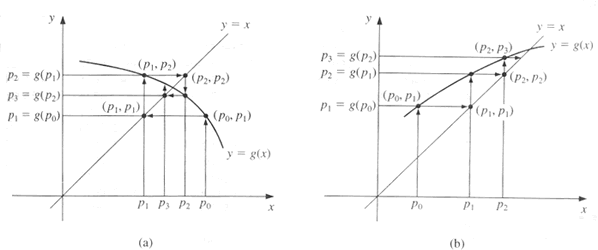
\includegraphics[width=400px]{img/PuntoFijo}

El siguiente teorema nos da algunas condiciones suficientes para
la convergencia del algoritmo de punto fijo para un valor inicial escogido en
un intervalo apropiado:

Sea $g(x)$ una función continua en un intervalo $[a, b]$ tal que
$g(x) \in [a,b] \; \; \forall x \in [a,b]$, entonces $g(x)$, tiene un punto
fijo $p$ en $[a, b]$ .

Si además, $g^\prime (x) $ existe en $]a,b[$ y es posible hallar una constante
$k<1$ tal que $g^\prime (x) \leq k, \; \mbox{para todo } x \in ]a,b[$,
entonces el punto fijo de $g(x)$en $[a, b]$ es único.

Adicionalmente, si $g^\prime (x) $ es continua en $]a,b[$ y $g^\prime (p) \neq
0$, entonces para cualquier valor inicial $x_0 \in [a, b]$, la sucesión
definida por
\begin{displaymath}x_{n+1}=g(x_n)\end{displaymath}
 
converge a $p$ y $\vert x_{n+1}-p\vert<k\vert x_n-p\vert$
